\documentclass{article}

\usepackage[T1]{fontenc}
\usepackage[english]{babel}
\usepackage[utf8]{inputenc}
\usepackage{vhistory}
\usepackage{graphicx}
\usepackage{listings}

\def\version {1.0.0}

\title{Gerrit \\ Quick start \\ \small{v\version}}

\author{Paweł Warzecha}
\date{\today}



\begin{document}

\maketitle

\newpage

\section{Introduction}

Gerrit is a free, web-based team code collaboration tool. Software developers in a team can review each other's modifications on their source code using a Web browser and approve or reject those changes. It integrates closely with Git, a distributed version control system. Gerrit is a fork of Rietveld, another code review tool. Both namesakes are of Dutch designer Gerrit Rietveld.\cite{Gerrit}

\section{Using Gerrit}

For this project we use GerritHub\cite{GerritHub}. It offers free and preconfigured Gerrit server. It has been chosen because it is a ready to use solution, widely used and integrated with the GitHub. 

Next sections show how to use Gerrit.

\subsection{Registering to GerritHub.io}

To use the GerritHub, the GitHub account is needed. If you don't have a GitHub account, create it first. Next if You don't have a GerritHub account click the ``First time Sign In'' button(marked with the red rectangle in the figure~\ref{fig:Register}). Next follow the instructions on the website.

\begin{figure}[!ht]
  \centering
  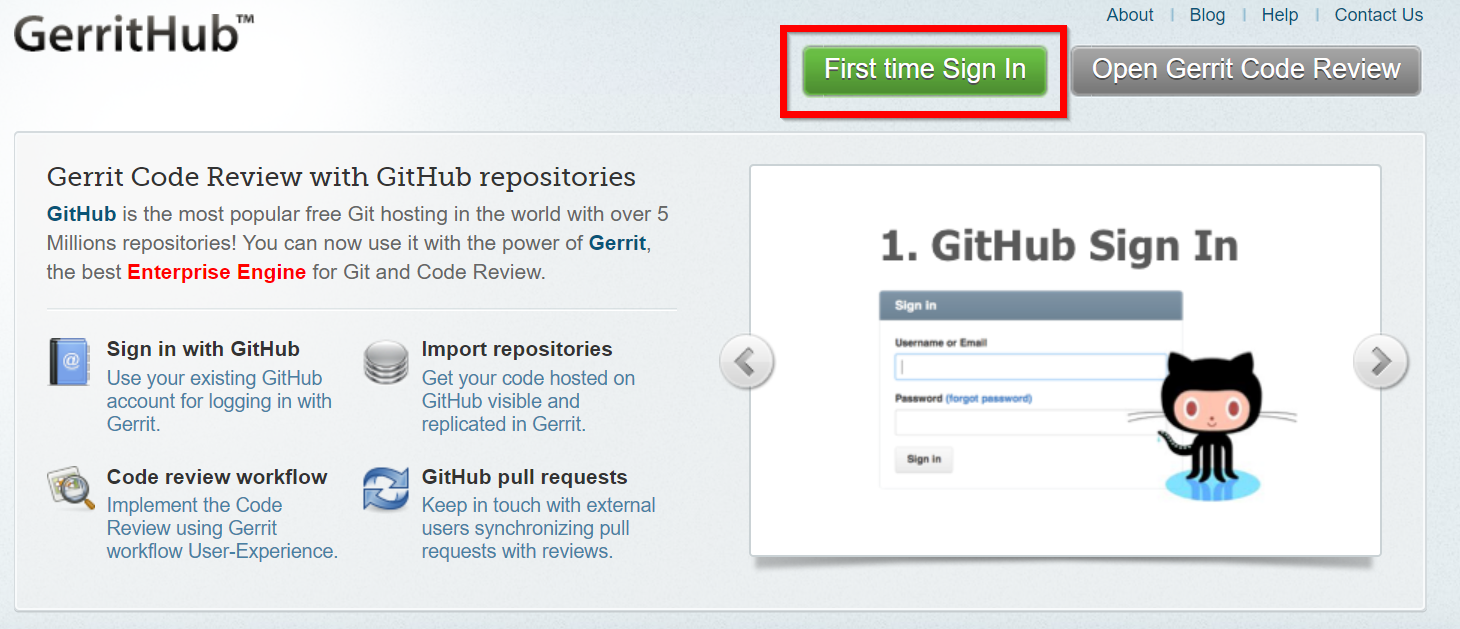
\includegraphics[width=.75\textwidth]{img/RegisterToGerritHub}
  \caption{Connecting github.}
  \label{fig:Register}
\end{figure}

\subsection{Cloning repository}

To clone the repository with the project code go to Browse->Projects and in the Filter write the name of the project in which you want to contribute (as shown in figure~\ref{fig:FindProject}). Next click on the project name.

\begin{figure}[!ht]
  \centering
  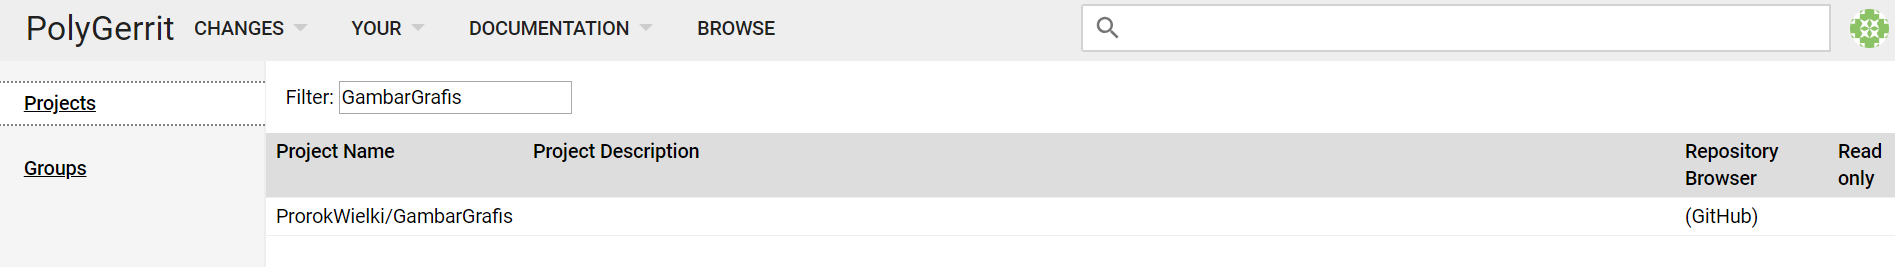
\includegraphics[width=.75\textwidth]{img/FindProject}
  \caption{Finding a project.}
  \label{fig:FindProject}
\end{figure}

On the site you can see the command which is needed to clone the repository (marked in figure~\ref{fig:Clone})

\begin{figure}[!ht]
  \centering
  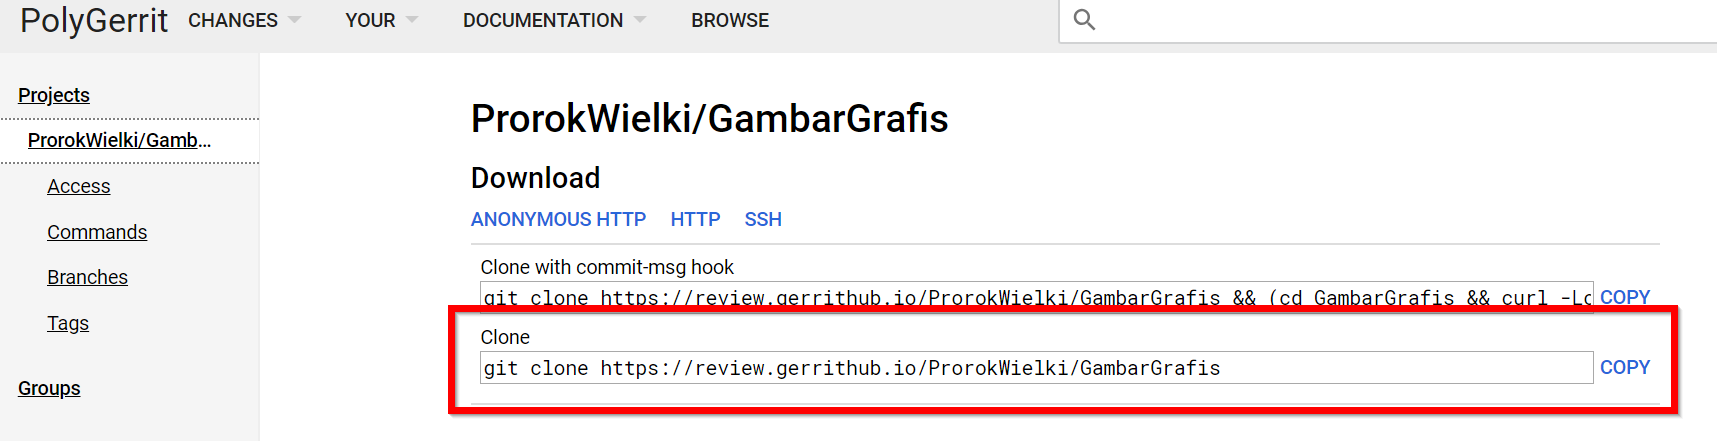
\includegraphics[width=.75\textwidth]{img/Clone}
  \caption{Clone command.}
  \label{fig:Clone}
\end{figure}

\subsection{Pushing changes}

If you want to push your changes to review, just use the git command, but change the branch name in the command to \textit{HEAD:refs/for/<branch\_name>} . For example, if you want to push the changes to a master branch use: 

\begin{lstlisting}
git push origin HEAD:refs/for/master
\end{lstlisting}

\subsubsection{Adding reviewer}

There are two ways to add reviewer(s) to your change. First, assigne the reviewer at the push. In this case use \textit{\%r=<email\_address>} at the end of the push command. The command may look like:

\begin{lstlisting}
git push origin HEAD:refs/for/master%r=ProrokWielki@o2.pl
\end{lstlisting}

The second way is to set the reviewer on the web site. In this case from \textit{YOUR->Changes} select the change to which you want to assign the reviewer. Then on the web page click \textit{ADD REVIEWER}. Put the reviewer email next to the \textit{Reviewers} (as shown in figure~\ref{fig:Reviewer})

\begin{figure}[!ht]
  \centering
  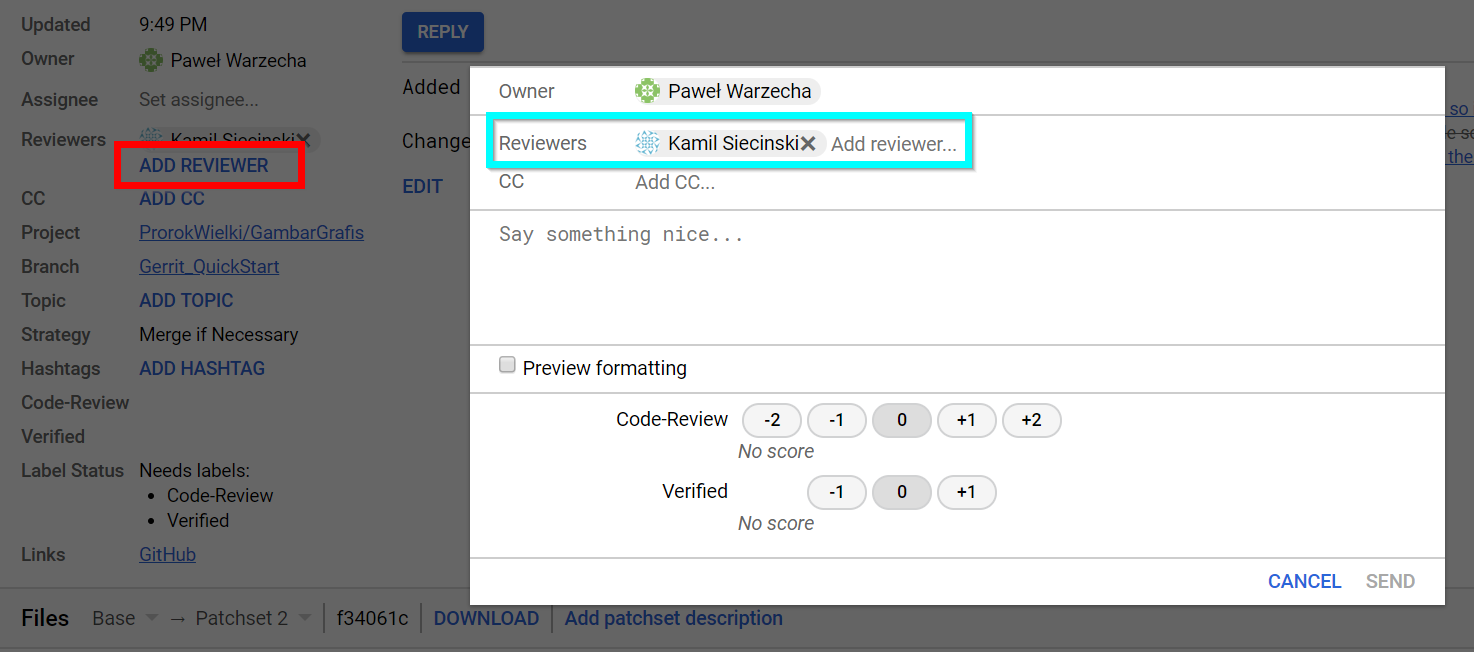
\includegraphics[width=0.75\textwidth]{img/Reviewer}
  \caption{Adding Reviewer.}
  \label{fig:Reviewer}
\end{figure}

\subsection{Reviewing change}

If you are asked to review someones change you can see that change in the \textit{Incoming reviews} in the \textit{YOUR->Changes} section.

In the Files Section you can find the files which were pushed with the change. To see the content of a file, click on its name.

\newpage

\begin{thebibliography}{9}

\bibitem{Gerrit} 
\textit{Wikipedia -- Gerrit (software)}.\\ 
\url{https://en.wikipedia.org/wiki/Gerrit_(software)}
 
\bibitem{GerritHub} 
\textit{GerritHub.io}.\\ 
\url{http://gerrithub.io/}

\end{thebibliography}

\newpage

\begin{versionhistory}
  \vhEntry{1.0.0}{22.01.04}{PW}{Created}
\end{versionhistory}

\end{document}
